\section{Deployment Plan}\label{sec:deployment}

Producing templates at survey scale requires many processing steps and substantial data movement, the quality of the output varies across the sky, and the templates must integrate cleanly with the existing LSSTCam template workflow in PP. The campaign therefore proceeds in discrete stages, so that templates are deployed for regions where they are ready, while later regions are still being processed or validated. The regular-processing deployment described here is distinct from the use of DECam templates for ToO analyses. It covers the templates used by PP for real-time alert production, with the expectation that deployment proceeds chunk by chunk as each chunk is processed and vetted.

Chunks are processed with a priority assigned based on field availability. For this reason, we initiated the processing campaign with templates within the DELVE footprint along an RA$=315^\circ$. This region was given priority given the original start date of LVK IR1, which was mid-November 2026\footnote{Note: The announced start date of LVK IR1 as of \today\ is \href{https://observing.docs.ligo.org/plan/\#ligo-virgo-and-kagra-observing-run-plans}{mid-January 2027}}, and the fields available to Rubin at that time. For this reason, we define chunk 0 as the chunk centered at RA$=315^\circ$, DEC$=+15^\circ$, shown in Figure~\ref{fig:chunk_schem}.

\begin{figure}[b!]
     \centering
     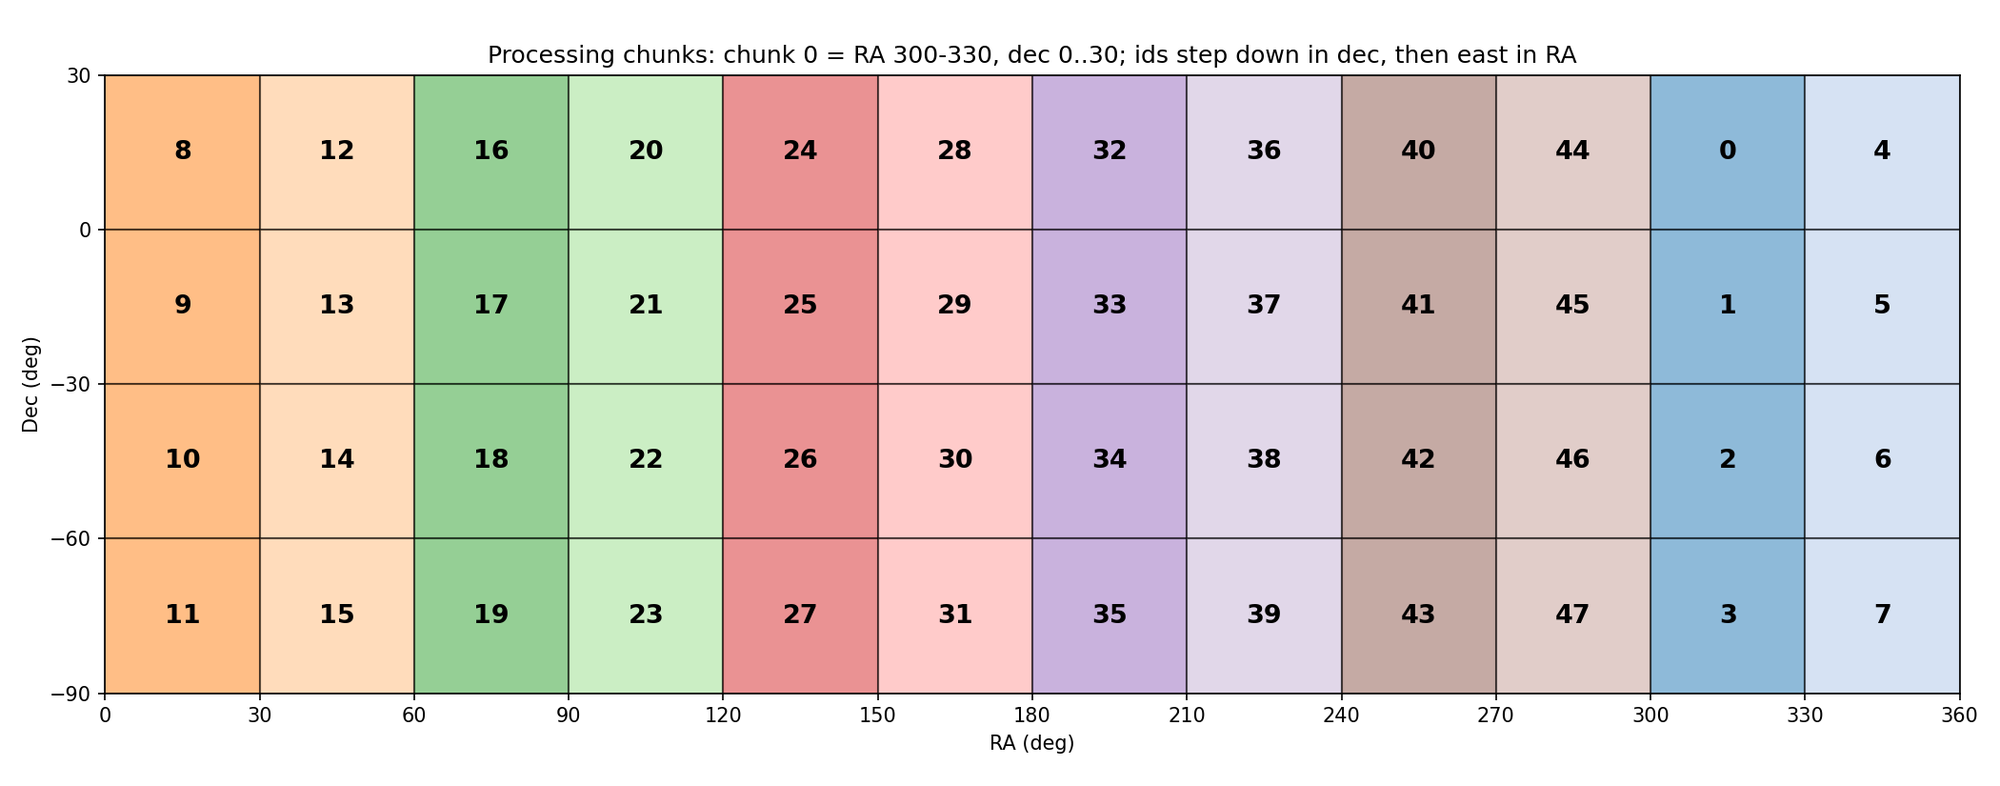
\includegraphics[width=\linewidth]{figures/chunk_schematic.png}
     \caption{A schematic of the chunks across the sky, illustrating the staging of template production and deployment.}
     \label{fig:chunk_schem}
 \end{figure}

\subsection{Transition to LSSTCam templates}

DECam templates are a stopgap, so the deployment plan includes their eventual replacement. As LSSTCam accumulates enough images in a tract and band, a decision is needed on when that tract and band switches from a DECam template to an LSSTCam template. Because only one style of template exists in the official chain for a given tract and band, the switch is a curation step rather than a runtime choice. \cite{RTN-133} quantifies how the benefit of DECam templates depends on the open choices: the number of visits per LSSTCam template, the latency of template builds, the image-quality cuts on the LSSTCam visits, and the time at which a tract switches from DECam to LSSTCam. The metadata recorded during coaddition is intended to allow a balanced mixture of DECam and LSSTCam templates as this transition progresses.

\subsection{Data retention and archiving}
\label{sec:archiving}

We archive \texttt{template\_coadd}, \texttt{preliminary\_visit\_image}, and \texttt{preliminary\_visit\_summary} datasets to tape at NERSC for each chunk, in the event of re-processing or data reuse for other scientific applications.

\subsection{Current status}

As of \today, chunk~0 (about 500\,deg$^2$) has been produced at NERSC, transferred to the USDF, vetted, re-ingested under the PP-required dataset type, and chained into the curated collection, with tracts and bands overlapping existing LSSTCam coverage removed. The remaining steps for chunk~0 are the transfer to \texttt{embargo}, which requires adjusting file ownership so that the PP service account can create the links, and configuring PP to use the new collection. Processing of other chunks is underway. The status of chunk processing is shown in Table ~\ref{tab:chunks}.

\begin{longtable}{c c c p{2cm} p{2cm} p{3cm}}
\caption{The status of chunk processing, as of \procDate}\label{tab:chunks}\\
\toprule
Chunk & RA range (deg) & Dec range (deg) & Area (deg$^2$) & MJD range (per band) & Expected date of transfer to USDF \\
\midrule
\endfirsthead
\toprule
Chunk & RA range (deg) & Dec range (deg) & Area (deg$^2$) & MJD range (per band) & Expected date of transfer to USDF \\
\midrule
\endhead
\midrule
\multicolumn{6}{r}{\emph{Continued on next page}} \\
\endfoot
\bottomrule
\endlastfoot
0  & 300--330 & $0$ to $30$    & & & \\
1  & 300--330 & $-30$ to $0$   & & & \\
2  & 300--330 & $-60$ to $-30$ & & & \\
3  & 300--330 & $-90$ to $-60$ & & & \\
4  & 330--360 & $0$ to $30$    & & & \\
5  & 330--360 & $-30$ to $0$   & & & \\
6  & 330--360 & $-60$ to $-30$ & & & \\
7  & 330--360 & $-90$ to $-60$ & & & \\
8  & 0--30    & $0$ to $30$    & & & \\
9  & 0--30    & $-30$ to $0$   & & & \\
10 & 0--30    & $-60$ to $-30$ & & & \\
11 & 0--30    & $-90$ to $-60$ & & & \\
12 & 30--60   & $0$ to $30$    & & & \\
13 & 30--60   & $-30$ to $0$   & & & \\
14 & 30--60   & $-60$ to $-30$ & & & \\
15 & 30--60   & $-90$ to $-60$ & & & \\
16 & 60--90   & $0$ to $30$    & & & \\
17 & 60--90   & $-30$ to $0$   & & & \\
18 & 60--90   & $-60$ to $-30$ & & & \\
19 & 60--90   & $-90$ to $-60$ & & & \\
20 & 90--120  & $0$ to $30$    & & & \\
21 & 90--120  & $-30$ to $0$   & & & \\
22 & 90--120  & $-60$ to $-30$ & & & \\
23 & 90--120  & $-90$ to $-60$ & & & \\
24 & 120--150 & $0$ to $30$    & & & \\
25 & 120--150 & $-30$ to $0$   & & & \\
26 & 120--150 & $-60$ to $-30$ & & & \\
27 & 120--150 & $-90$ to $-60$ & & & \\
28 & 150--180 & $0$ to $30$    & & & \\
29 & 150--180 & $-30$ to $0$   & & & \\
30 & 150--180 & $-60$ to $-30$ & & & \\
31 & 150--180 & $-90$ to $-60$ & & & \\
32 & 180--210 & $0$ to $30$    & & & \\
33 & 180--210 & $-30$ to $0$   & & & \\
34 & 180--210 & $-60$ to $-30$ & & & \\
35 & 180--210 & $-90$ to $-60$ & & & \\
36 & 210--240 & $0$ to $30$    & & & \\
37 & 210--240 & $-30$ to $0$   & & & \\
38 & 210--240 & $-60$ to $-30$ & & & \\
39 & 210--240 & $-90$ to $-60$ & & & \\
40 & 240--270 & $0$ to $30$    & & & \\
41 & 240--270 & $-30$ to $0$   & & & \\
42 & 240--270 & $-60$ to $-30$ & & & \\
43 & 240--270 & $-90$ to $-60$ & & & \\
44 & 270--300 & $0$ to $30$    & & & \\
45 & 270--300 & $-30$ to $0$   & & & \\
46 & 270--300 & $-60$ to $-30$ & & & \\
47 & 270--300 & $-90$ to $-60$ & & & \\
\end{longtable}